\subsubsection{State Charts}
In this section are illustrated the state charts of classes Tournament and Battle, to show the different states of these classes, and all possible transitions.\\

\textbf{Tournament State Chart:}
\begin{figure}[h]
    \centering
    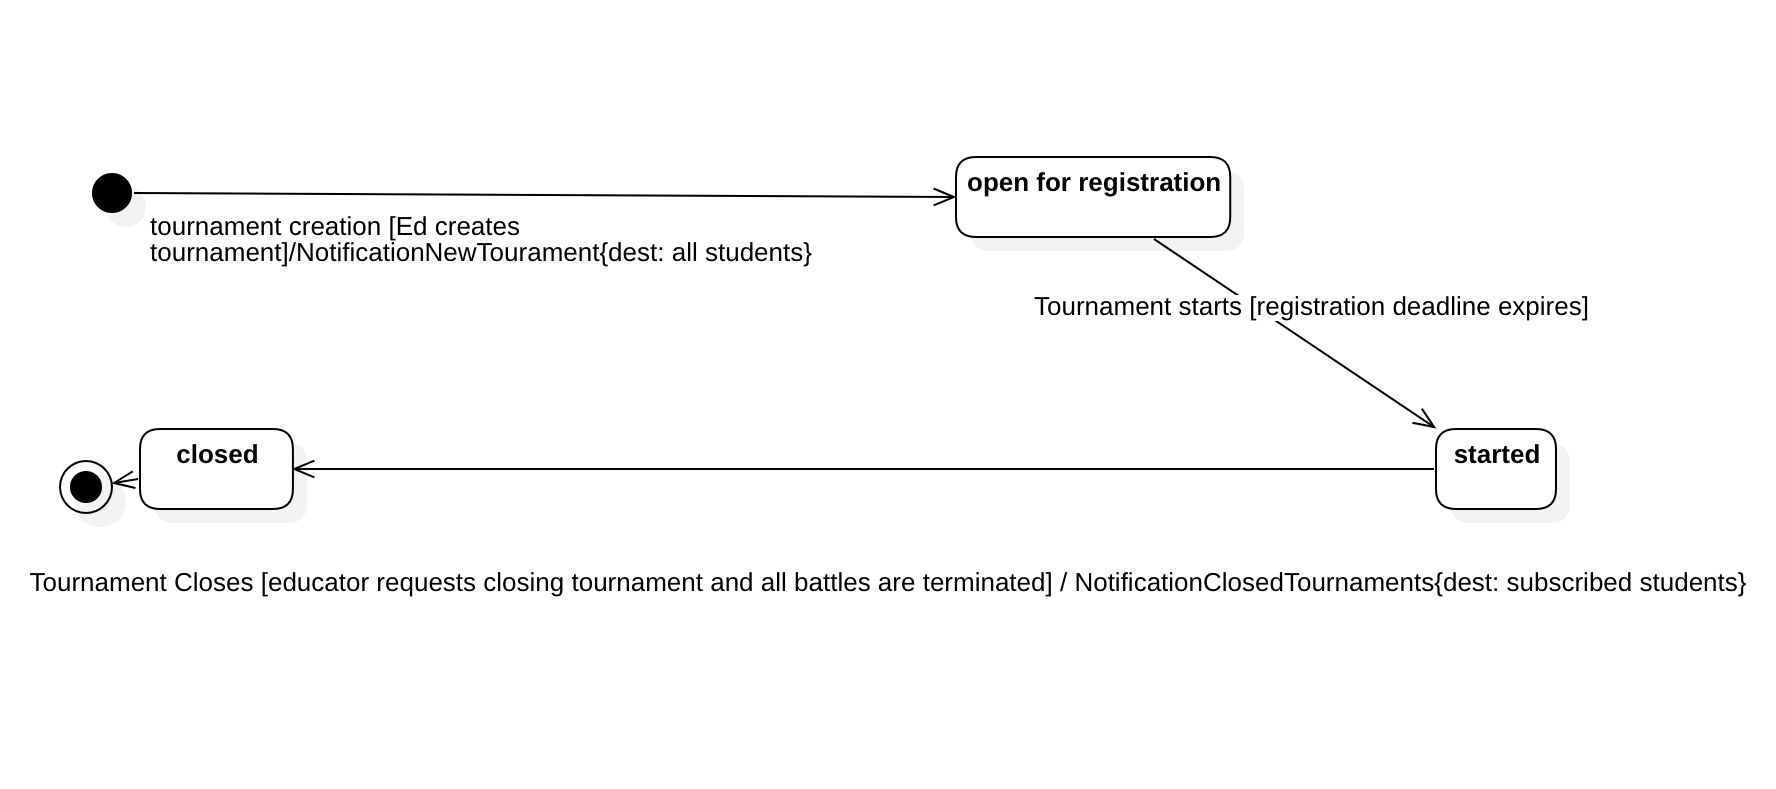
\includegraphics[width=1\textwidth]{2Overall_Description/res/st1.png}
\end{figure}

After an educator has created a tournament all the students can subscribe to it, this is the \textbf{Open for registration} state. After the registration deadline the tournament starts, student can't enroll anymore and edcucators can create battles, this is the \textbf{Started} state. When the educator that created the tournament decides it's time to close it, he can do so if there aren't ongoing battles, if he succeeds the tournament is closed (state \textbf{closed}).\\
\\
\clearpage
\textbf{Battle State Chart:}
\begin{figure}[h]
    \centering
    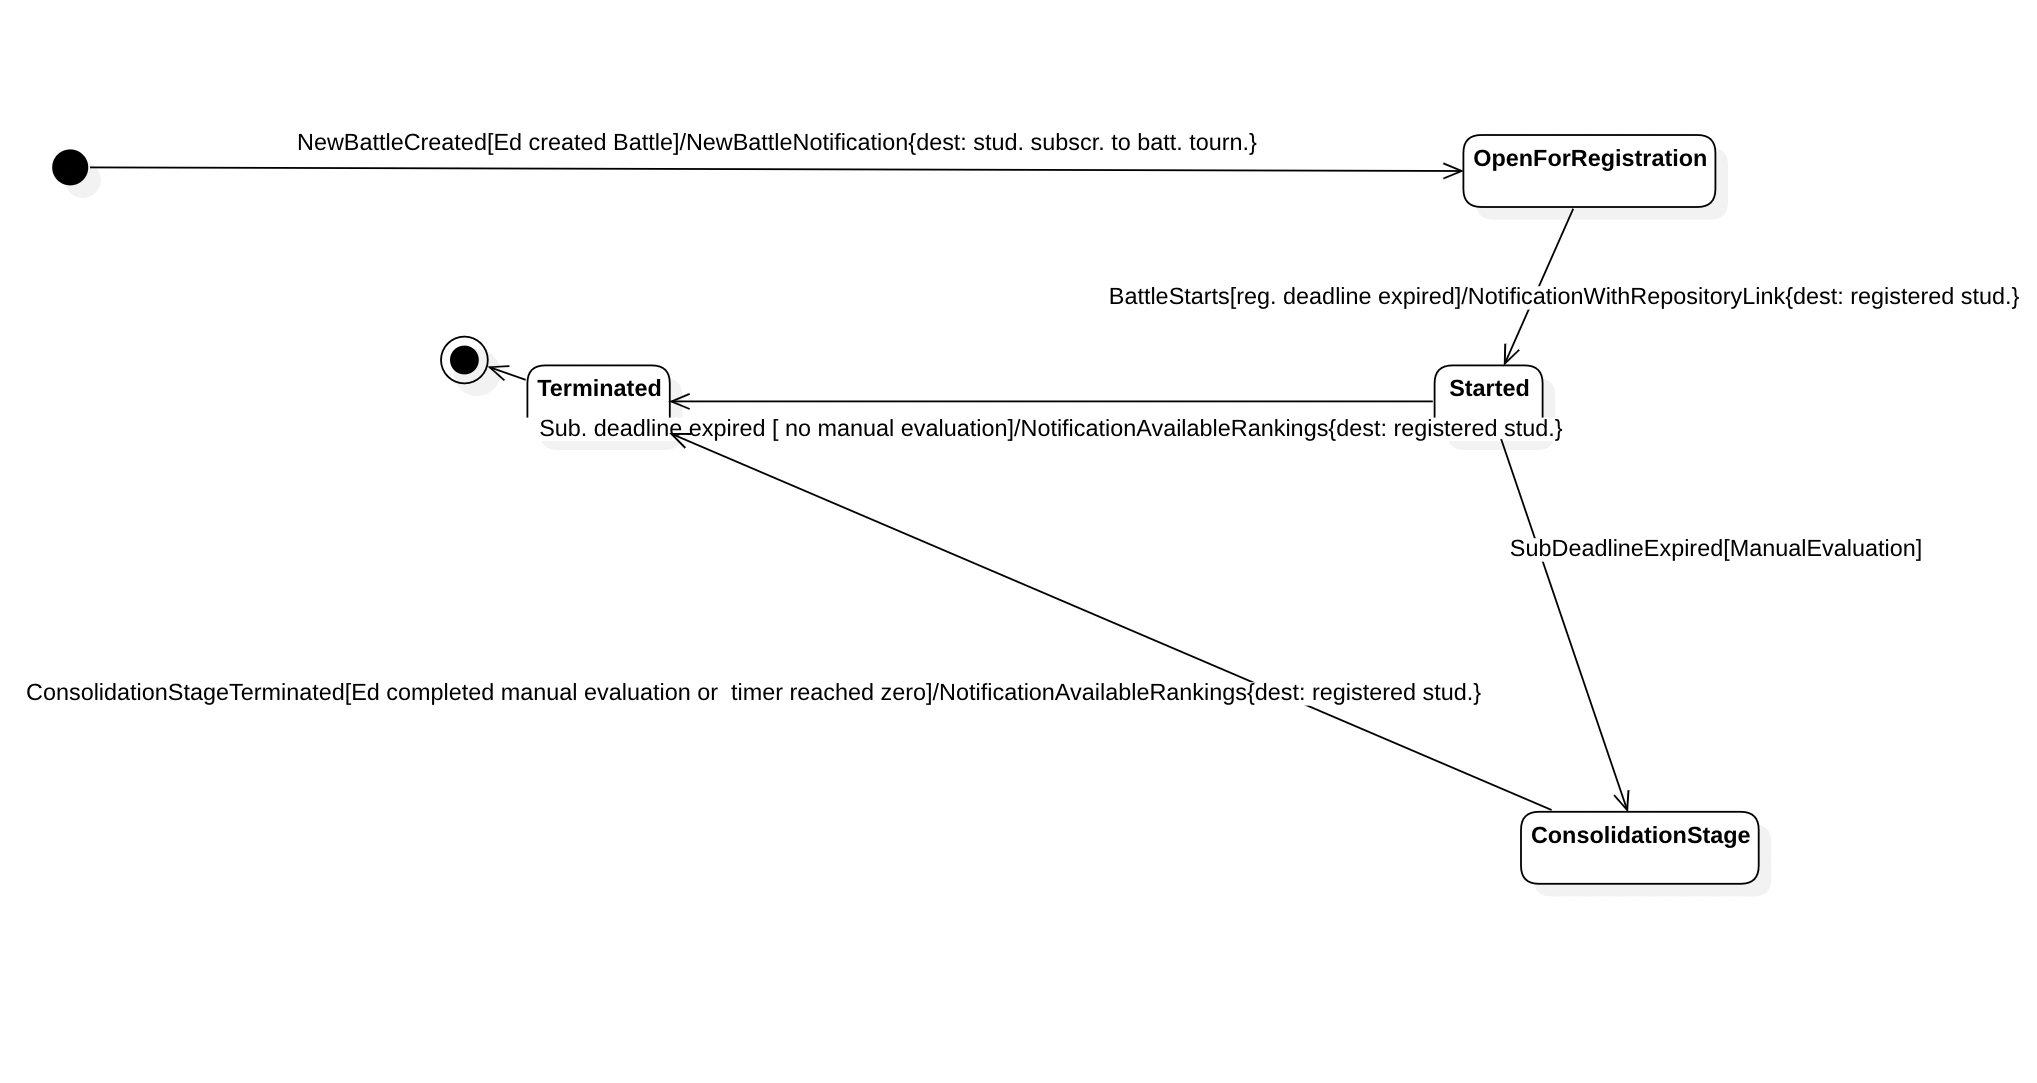
\includegraphics[width=1\textwidth]{2Overall_Description/res/stateChartBattle.png}
\end{figure}

After a battle is created students can enroll (\textbf{Open for registration} state). After the registration deadline students can't enroll anymore and a link to the battle repository is sent to all the registered students, (\textbf{Started} state). After the submission deadline, if the educator who created the battle has included a manual evaluation the Battle goes in a \textbf{Consolidation Stage} state. During the consolidation stage the educator assigns a score to each team last updated solution. The Battle goes from the consolidation stage state to \textbf{Terminated} state when the educator has finished grading all solutions, or when too much time has passed since the consolidation stage has started (fixed at 30 days). If no manual evaluation is expected, when the submission deadline expires the battle goes from the state \textbf{Started} to state \textbf{Terminated}.
\clearpage

\subsubsection{Activity Diagrams}
Here are illustrated the activity diagrams of the important workflows of CKB we wanted to highlight.\\
\\
\textbf{Computing Score Activity Diagram}\\
\begin{figure}[h]
    \clearpage
    \centering
    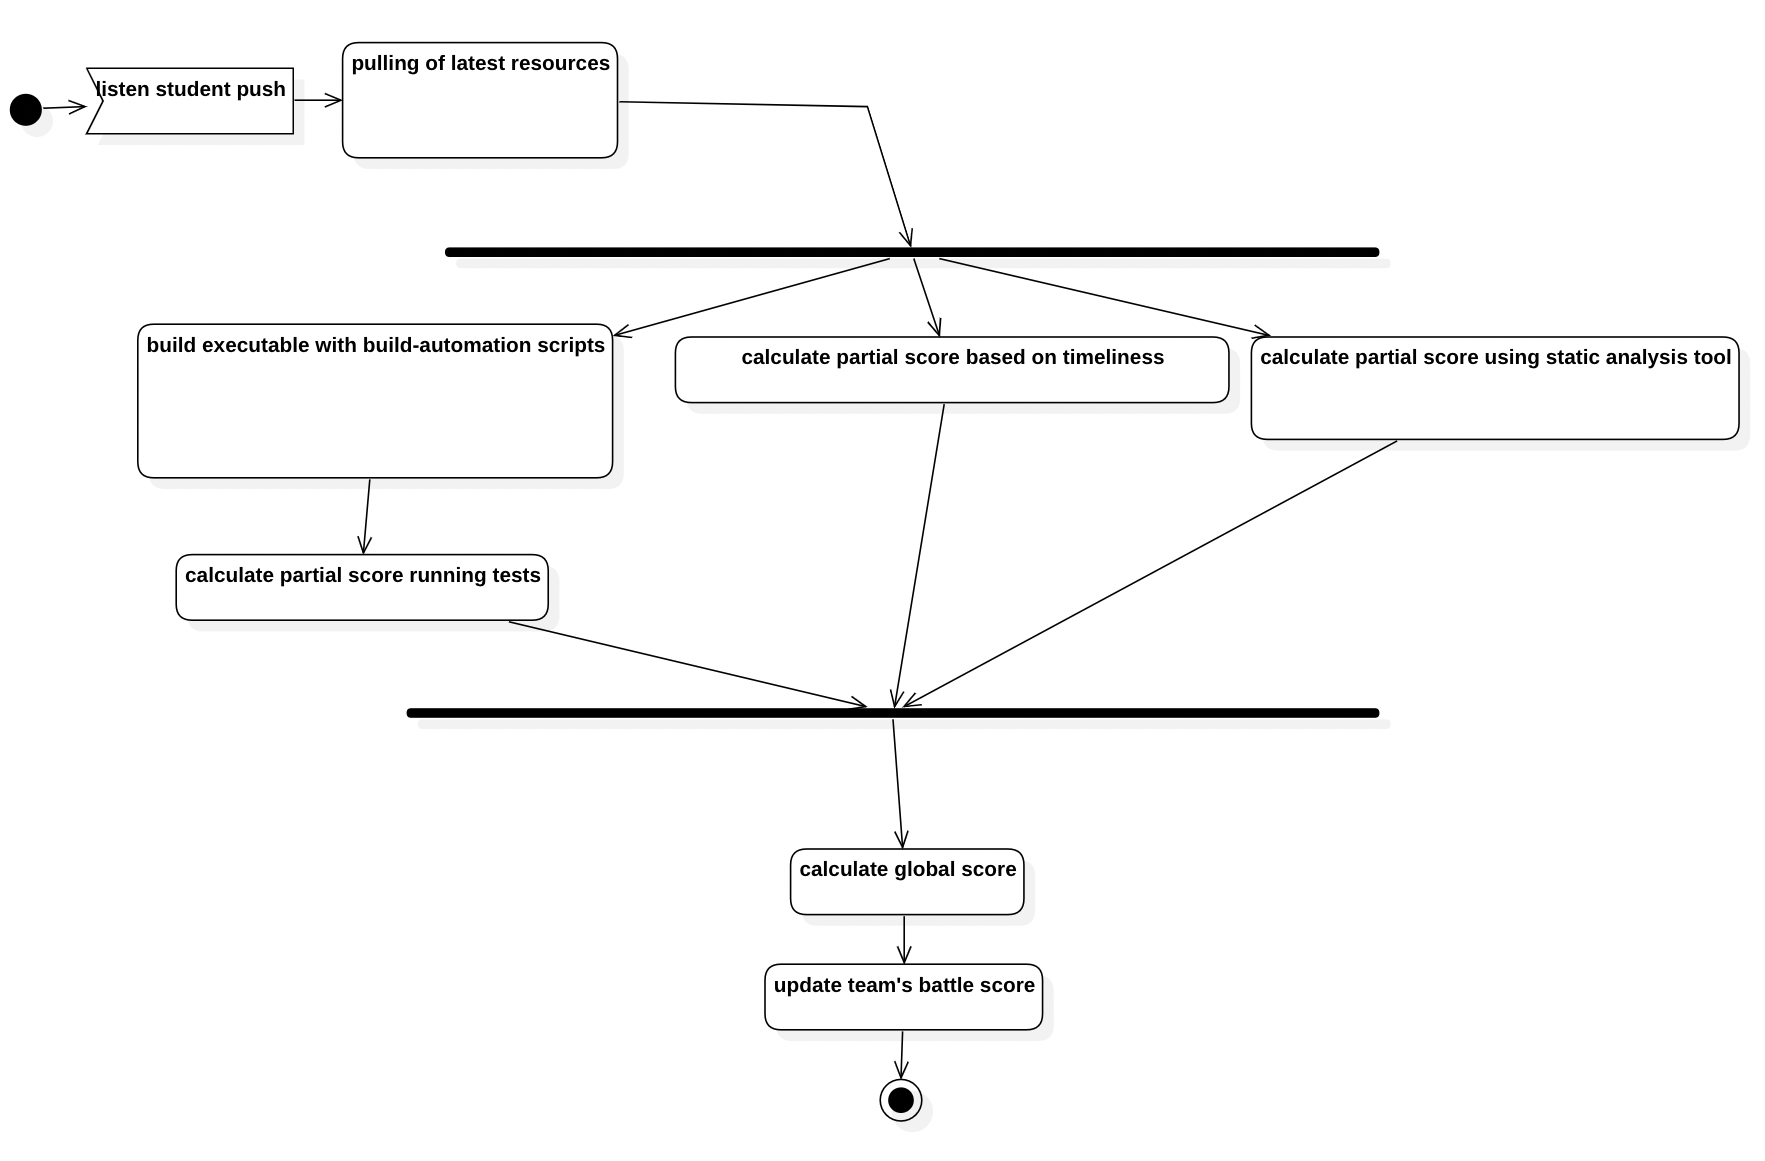
\includegraphics[width=1\textwidth]{2Overall_Description/res/newestActDgPush.png}
\end{figure}

The first activity diagram regards the process of anlayzing the correctnenss of a team's solution and the computation of it's score. The process is triggered by a push made by a student in the main branch of his ForkedRepository. Since the final score is obteined by merging results of three different analysis (static analysis, timeliness and number of test cases passed) we modeled the activities as three parallel activities.\\
\\
\newpage
\textbf{End of Battle Activity Diagram}\\
\begin{figure}[h]
    \centering
    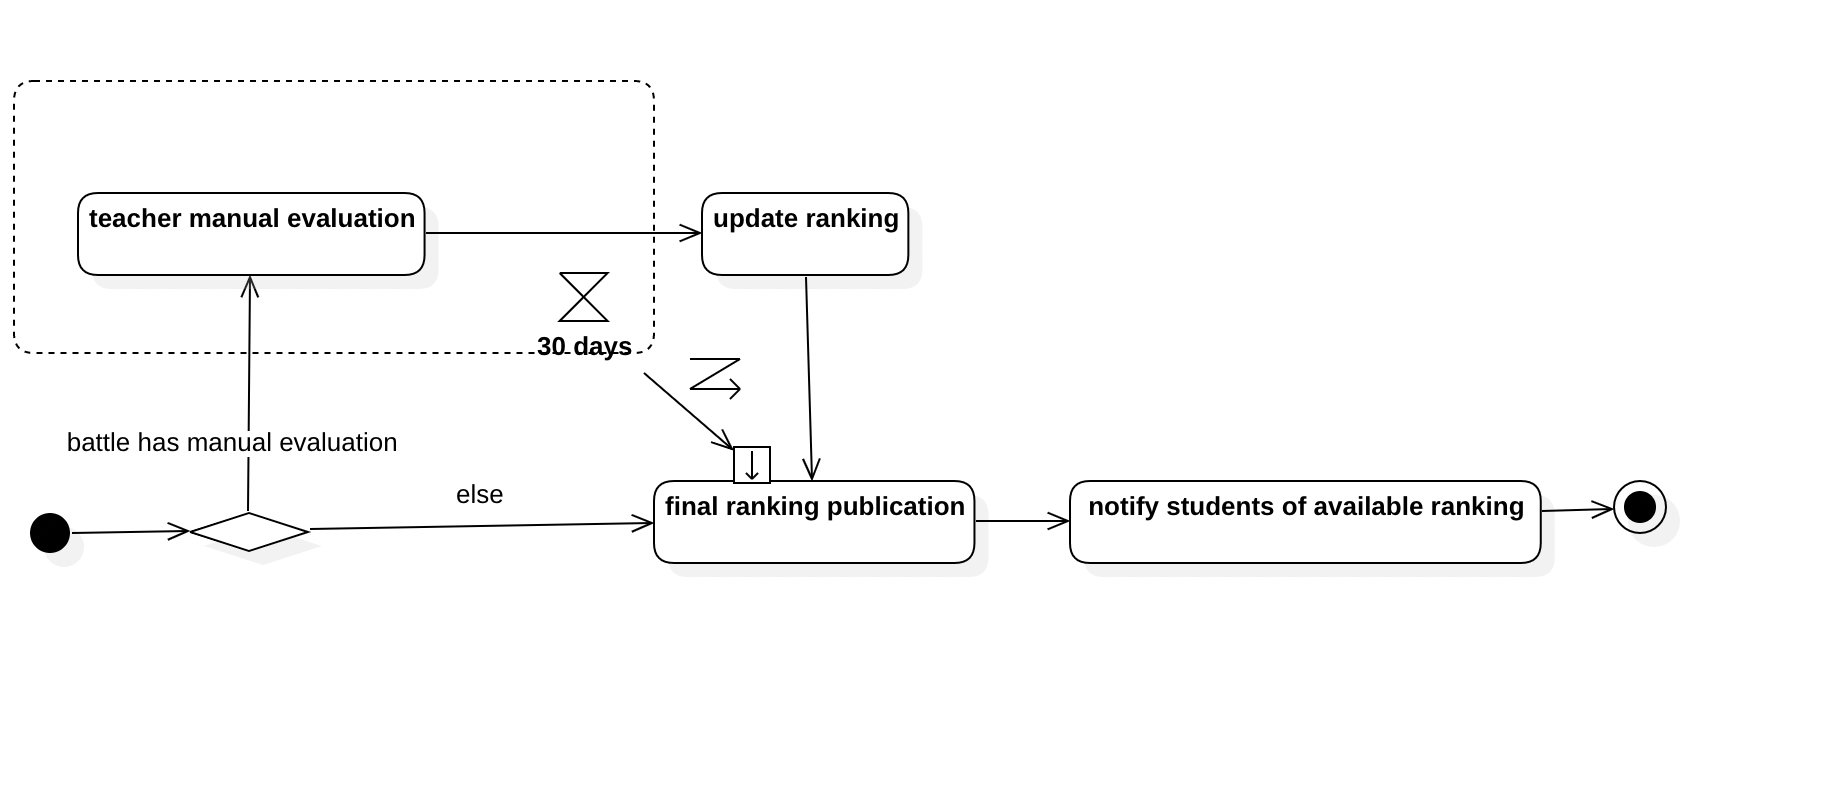
\includegraphics[width=1\textwidth]{2Overall_Description/res/ActivityDiagramEndBattle.png}
\end{figure}

The second activity diagram delineates the process of publishing the conclusive battle results, initiated upon the expiration of the battle submission deadline. The diagram is of interest because it highlights the workflow of when a battle expects a manual evaluation. The  \textbf{Manual Evaluation} activity is executed by an external actor, typically an educator. Should this activity not conclude before a predefined time, the system autonomously proceeds to publish the final results.
